\section{Metriken zur Bewertung von Multi-Object Tracking Systemen} \label{sec:MOT Metrics}

Maschinelles Lernen benötigt Merkmale, mit deren Hilfe Zusammenhänge verschiedener Aspekte eines Sachverhalts erlernt werden können. Ein Beispiel ist die Schätzung von Verkaufswerten von Autos. Relevante Merkmale können dafür die Kilometeranzahl, das Alter und die Marke sein. Solche Merkmale werden Features genannt. Aus den Trajektorien, die ein MOT System generiert, sollen Features extrahiert werden, die das individuelle Verhalten der Tiere verwertbar machen für maschinelles Lernen. Um sicherzustellen, dass sich aus den generierten Trajektorien tatsächlich nützliche Features extrahieren lassen, wird das MOT System evaluiert. In diesem Kapitel wird das Grundlagenverständnis für die Evaluation geschaffen und anschließend werden drei Verfahren im Detail betrachtet. \par

So wie \gls{MOT} selbst ist auch die Bewertung von \gls{MOT} Systemen ein recht junges Feld. In den vergangenen Jahren wurden einige Verfahren und Metriken für diesen Zweck entwickelt, jedoch hat sich davon keine deutlich gegenüber den anderen durchgesetzt, weshalb in Veröffentlichungen oftmals mehrere Metriken angegeben werden. Deswegen werden auch hier drei Metriken vorgestellt. Geordnet sind sie in ihrer historischen Reihenfolge. Während die  \textit{\acrshort{CLEAR} \gls{MOT}} Metriken \cite{CLEAR.2008} und die \textit{\gls{IDF1}-Metrik} \cite{IDF1} sich inzwischen etabliert haben, ist die \gls{HOTA} \cite{HOTA} der neuste Ansatz von den Dreien und noch weniger etabliert. Bevor die einzelnen Metriken im Detail vorgestellt werden, wird auf einige Grundlagen der Evaluation von \gls{MOT} Systemen eingegangen.

\subsection{Grundlagen der Bewertung von Multi-Object Tracking Systemen} \label{sec:MOT GT}
Die Evaluation von \gls{MOT} Systemen funktioniert über ein \glsdisp{Ereignis}{Referenzereignis}. Diese Referenz beinhaltet alle korrekten \gls{Detektion}[en], \gls{Lokalisation}[en] und \gls{Assoziation}[en]. Diese Referenz wird als \gls{Ground Truth} bezeichnet \cite{HOTA}. Das \gls{MOT} System wird auf das \glsdisp{Ereignis}{Referenzereignis} angewendet und gibt ein Ergebnis zurück. Dieses Ergebnis wird mit der \gls{Ground Truth} verglichen. Der Grad der Übereinstimmung ist das Evaluationsergebnis für das \gls{MOT} System. Die verschiedenen Metriken unterscheiden sich in ihrer Berechnung des Übereinstimmungsgrads. Dadurch kommt es zu Unterschieden in der Gewichtung des Einflusses der Fehlertypen (\autoref{sec:MOT Fehlertypen}) und der \gls{Modul}[e] von \gls{MOT} Systemen \cite{HOTA, IDF1, CLEAR.2008}.\par

Für eine aussagekräftige Evaluation wird eine qualitativ hochwertige \gls{Ground Truth} benötigt. Diese zu erstellen, ist jedoch eine herausfordernde Aufgabe. Die Erstellung einer \gls{Ground Truth} erfolgt manuell und ist oftmals zeitaufwendig. Ebenfalls kommt es bei \gls{MOT} Problemen häufig zu Mehrdeutigkeiten, welche selbst für einen Menschen nicht lösbar sind. Beispiele hierfür sind Spiegelungen in Fensterscheiben. Die Frage, die in dieser Situation zu beantworten ist, wäre, ob eine Spiegelung vom \gls{MOT} System als Objekt erkannt werden soll, oder ob es ein Fehler ist, wenn es das tut. Auch der Umgang mit teilweisen Verdeckungen ist nicht eindeutig zu lösen. Solche Probleme treten oft in den Randbereichen des Kameraausschnitts auf, da hier beim Verlassen oder Eintreten in das Bild das Objekt nur teilweise sichtbar ist. Ab wann bzw. bis wann in diesem Fall ein Objekt zu \glsdisp{Detektion}{detektieren} ist, ist nicht eindeutig lösbar. Auch bei der manuellen \gls{Lokalisation} kommt es zu Abweichungen durch menschliche Fehler \cite{MOT15, Milan.2013}.  \par

Aus diesen Gründen ist es nicht möglich eine ideale \gls{Ground Truth} ohne Fehler und Varianz zu erstellen. Um dennoch eine aussagekräftige Evaluation zu erhalten, wird empfohlen, mehrere \glsdisp{Ereignis}{Referenzereignis} zu erstellen und die Ergebnisse zu mitteln \cite{Milan.2013}. Ebenfalls hilft es vor der \gls{Ground Truth} Erstellung klare Regeln zu definieren, wie mit Mehrdeutigkeiten und anderen Herausforderungen umzugehen ist. Solche definiert auch die \textit{MOTChallenge} \cite{MOT16, MOT20}. Die \textit{MOTChallenge} ist ein regelmäßiger Wettbewerb für \gls{MOT} Systeme und hat sich zur Aufgabe gemacht, eine Benchmark für diese Systeme zu schaffen. Für das Benchmarking stehen mehrere \gls{Ground Truth} Datensätze zur Verfügung, welche alle nach den gleichen Regeln erstellt worden sind. Für das \gls{Detektion}[s]- und das \gls{Lokalisation}[s]\glsdisp{Modul}{modul} eines \gls{MOT} System werden oftmals Trainingsdaten benötigt. Die \textit{MOTChallenge} stellt dazu Trainingsdaten zur Verfügung, die nach den gleichen Regeln geschaffen wurden, wie die \gls{Ground Truth} \cite{MOT16, MOT20}. Dies ermöglicht eine faire Bewertung für das \gls{Detektion}[s]- und das \gls{Lokalisation}[s]\glsdisp{Modul}{modul}. Wäre dies nicht der Fall, kann es sein, dass das System einen anderen Umgang mit den Herausforderungen und Mehrdeutigkeiten gelernt hat, als es die \gls{Ground Truth} erwartet. Dadurch können Ergebnisse verzerrt werden. \par

Der Fokus der \textit{MOTChallenge} liegt primär auf dem \gls{Tracking} von Fußgängern. Dafür stellt der Wettbewerb Trainings- und Testdatensätze zur Verfügung, um diese Prozesse bei allen teilnehmenden Systemen zu vereinheitlichen. Dies zeigt jedoch, dass ein aussagekräftiger Vergleich von \gls{MOT} Systemen, bezogen auf eine konkrete Anwendung, nur mit einheitlichen Trainings- und Testdatensätzen möglich ist. Werden für einen Anwendungsfall, wie z.B. das \gls{Tracking} von Fahrzeugen im Straßenverkehr, unterschiedliche Systeme mit unterschiedlichen Datensätzen beurteilt, dann sorgen die Herausforderungen der \gls{Ground Truth} Erstellung dafür, dass die Vergleichbarkeit der Ergebnisse nur eingeschränkt gegeben ist \cite{MOT15}. 

\subsection{Die CLEAR MOT Metriken} \label{sec:MOT MOTA}
Die \textit{\acrshort{CLEAR} \gls{MOT}} Metriken sind einer der ersten Versuche, einheitliche und allgemeine Metriken für die Bewertung von \gls{MOT} Systemen zu schaffen. Vor ihrer Veröffentlichung gab es keine Methode, die sich für diese Aufgabe durchsetzen konnte. Bis heute ist sie eine der verbreitetsten Metriken für \gls{MOT} Systemen. In \cite{CLEAR.2008} werden zwei Metriken vorgestellt. In \cite{Kasturi.2009} werden diese um weitere Metriken ergänzt. \par

Um die \textit{\acrshort{CLEAR} \gls{MOT}} Metriken berechnen zu können, wird eine \gls{Ground Truth} benötigt und das \gls{Tracking}[ergebnis] eines \gls{MOT} Systems. Die \gls{Detektion}[en] des \gls{Tracking}[ergebnisses] sind die Menge \(SysDet = \{sysDet_1, sysDet_2, \dots, sysDet_n\}\). Sie müssen den korrekten \gls{Detektion}[en] aus der \gls{Ground Truth} \(GtDet = \{gtDet_1, gtDet_2, \dots, gtDet_n\}\) zugeordnet werden, um die Korrektheit des \gls{Tracking}[ergebnisses] beurteilen zu können. Dabei erfolgt die Zuordnung eins zu eins. Das bedeutet jedes Element \(gtDet_i \in GtDet\) bekommt maximal ein Element \(sysDet_j \in SysDet\) zugeordnet und in die andere Richtung genau so. Die Zuordnung erfolgt \glsdisp{Frame}{frameweise}. Um in einem \gls{Frame} eine \(gtDet_i\) zu einer \(sysDet_i\) zuzuordnen, wird eine minimale Ähnlichkeit \(\alpha\) zwischen den möglichen Zuordnungen verlangt. Bei \gls{Bounding Box}[en] lässt sich die Ähnlichkeit durch die \(\gls{IoU}\) ausdrücken. Die Schwelle \(\alpha\) ist vom Anwender festzulegen, da die Ähnlichkeitsanforderung für eine korrekte Zuordnung anwendungsspezifisch seien kann. Dies ist jedoch der einzige nicht allgemeine Parameter der \textit{\acrshort{CLEAR} \gls{MOT}} Metriken. Für die Zuordnung einer \(sysDet_i\) zu einer \(gtDet_i\) kommen alle \(sysDet_j \in SysDet\) infrage, die eine Ähnlichkeit \(s \geq \alpha\) besitzen. Von den \gls{Detektion}[en] \(sysDet_j \in SysDet\), welche diese Anforderung erfüllen, wird die \(sysDet_j\) bevorzugt, welche die \acrshort{ID} für das Objekt aus den vorherigen \gls{Frame}[s] konstant hält. Die Zuordnungsaufgabe der \(sysDet_j \in SysDet\) zu den  \(gtDet_i \in GetDet\), für die keine Zuordnungsoptionen bestehen, welche die \acrshort{ID}[s] konstant halten, wird global gelöst. Die globale Lösung versucht die Anzahl der \gls{Detektion}[sfehler] (\autoref{sec:MOT Fehlertypen}) zu minimieren und die Ähnlichkeit zu maximieren. Dies geschieht mit der ungarischen Methode \cite{Kuhn.1955}. Dieses Verfahren wirkt sich so auf die Metriken aus, dass diese maximal werden. \cite{CLEAR.2008, HOTA}. \par

Alle \(sysDet_i\), welche einer \(gtDet_i\) zugeordnet werden können, gelten als \glsdisp{EP}{echt positive Detektionen (EP)} des Systems. \(Det_{\gls{EP}_t}\) sind alle \glsdisp{EP}{echt positiven} \gls{Detektion}[en] zum Zeitpunkt \(t\). Alle \(gtDet_i\), welche keine Zuordnung erhalten haben, sind \glsdisp{FN}{falsch negativ} \(Det_{\gls{FN}_t}\) und alle \(sysDet_j\), welche keine Zuordnung erhalten haben sind \glsdisp{FP}{falsch positiv} \(Det_{\gls{FP}_t}\). Jedes mal, wenn ein Objekt der \gls{Ground Truth} vom System eine andere \acrshort{ID} erhält als in den \gls{Frame}[s] zuvor, wird dies als ein \gls{IDSW} gezählt. \(\gls{IDSW}_t\) ist die Menge der \gls{IDSW}[s] im Zeitpunkt \(t\). \(N\) ist die Menge der \gls{Frame}[s] im \gls{Ereignis} und für die Zeitpunkte gilt \(t \in N\). \cite{CLEAR.2008, IDF1}. \par

Auf Basis der Zuordnung von \gls{Ground Truth} und \gls{Tracking}[ergebnis] definiert \cite{CLEAR.2008} zwei Metriken: \gls{MOTP} und \gls{MOTA}. Im gleichen Zuge wird oftmals auch \gls{MODA} genannt \cite{Kasturi.2009}. 

\begin{equation}
    \label{eq:MOTA}
    MOTA = 1-\frac{\sum_{t=1}^{N} (Det_{\gls{FN}_{t}}+Det_{\gls{FP}_{t}}+|\gls{IDSW}_{t}|)}{\sum_{t=1}^{N}gtDet_t}
\end{equation}

Die \autoref{eq:MOTA} zeigt die Berechnung der \gls{MOTA} Wertung. Die Anzahl der \gls{Detektion}[sfehler] und die \gls{IDSW} werden über alle \gls{Frame}[s] \(N\) aufsummiert. Das Gleiche geschieht mit allen \(gtDets\). \gls{MOTA} bewertet somit kombiniert die \gls{Modul}[e] für die \gls{Assoziation} und die \gls{Detektion}. 

\begin{equation}
    \label{eq:MOTP}
    MOTP = \frac{\sum_{t=1}^{N}S_{\gls{EP}_t}}{\sum_{t=1}^{N}Det_{\gls{EP}_t}}
\end{equation}

Mittels der \autoref{eq:MOTP} lässt sich der \gls{MOTP} Wert berechnen. Dies erfolgt über die Aufsummierung der Ähnlichkeit aller \gls{EP} Paarungen und der Division durch die Anzahl der \gls{EP} Paarungen. Somit entspricht \gls{MOTP} dem arithmetischen Mittelwert der Ähnlichkeit. Es ist ein Maß für die Genauigkeit der \glsdisp{Lokalisationsfehler}{Lokalisation}.

\begin{equation}
    \label{eq:MODA}
    MODA =  1-\frac{\sum_{t=1}^{N} (Det_{\gls{FN}_{t}}+Det_{\gls{FP}_{t}})}{\sum_{t=1}^{N}gtDet_t}
\end{equation}

Wie die \autoref{eq:MODA} zeigt, handelt es sich um die gleiche Formel wie die \autoref{eq:MOTA} nur ohne Berücksichtigung der \gls{IDSW}[s]. Somit hat das \gls{Assoziation}[s]\glsdisp{Modul}{modul} keinen Einfluss auf die MODA Wertung. Es handelt sich bei der \autoref{eq:MODA} um eine reine Bewertung des \gls{Detektion}[s]\glsdisp{Modul}{moduls} \cite{CLEAR.2008, HOTA, Kasturi.2009}.


\subsection{Die Identifikationsmetrik: IDF1} \label{sec:MOT F1}
Die Motivation hinter der \textit{\gls{IDF1}-Metrik} ist, dass vorausgegangene Metriken, wie die \textit{\acrshort{CLEAR} \gls{MOT}} Metriken ein verzerrtes Bild entstehen lassen können, wenn es darum geht, welches \gls{MOT} System am besten für eine Aufgabe geeignet ist. Dies lässt sich an einem Beispiel demonstrieren. In einem Überwachungsszenario soll eine Person verfolgt werden. Ein \gls{MOT} System \(A\) weist der verfolgten Person die \acrshort{ID} \(a1\) zu und ist in der Lage, die Identität über zehn \gls{Frame}[s] konstant zu halten. Danach macht es einen \gls{IDSW} und die Person erhält die \acrshort{ID} \(a2\). Ein \gls{MOT} System \(B\) gibt der Person die \acrshort{ID} \(b1\) und hält diese ebenfalls für zehn \gls{Frame}[s] konstant. Anschließend wechselt das System die \acrshort{ID} der Person zwischen \(b1\) und \(b2\) hin und her. Die \autoref{fig:bspIDF1vsMOTA} veranschaulicht das Beispiel.

\begin{figure}[htb]
     \centering
     \begin{subfigure}[b]{0.49\textwidth}
         \centering
         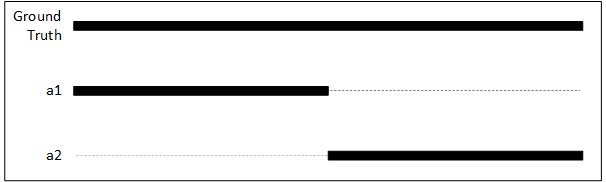
\includegraphics[width=\textwidth, height=3cm]{img/Grafiken/IDF1 bsp Motivation 1.png}
         \caption{Tracking des MOT Systems \(A\)}
     \end{subfigure}
     \hfill
     \begin{subfigure}[b]{0.49\textwidth}
         \centering
         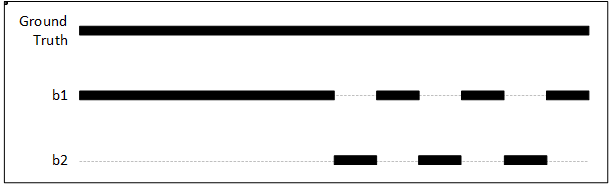
\includegraphics[width=\textwidth, height=3cm]{img/Grafiken/IDF1 bsp Motivation 2.png}
         \caption{Tracking des MOT Systems \(B\)}
     \end{subfigure}
     \caption[Beispiel zum Ansatz der \textit{\gls{IDF1}-Metrik}.]{Beispiel zum Ansatz der \textit{\gls{IDF1}-Metrik}. Vergleich zweier MOT System \cite{HOTA}.}
     \label{fig:bspIDF1vsMOTA}
\end{figure}

Wenn nun für diesen Anwendungsfall eins der beiden \gls{MOT} Systeme auszuwählen ist, dann würde die Wahl auf \(B\) fallen, da die verfolgte Person auch nach den ersten zehn \gls{Frame}[s] auffindbar ist, wenn auch nicht konstant. \gls{MOTA} würde jedoch das \gls{MOT} System \(A\) höher bewerten, da es nur einen \gls{IDSW} macht. Die \textit{\gls{IDF1}-Metrik} hält es für sinnvoller, zu bewerten, wie gut ein \gls{MOT} System darin ist, Identitäten korrekt zuzuweisen \cite{IDF1}. \par

Für die Berechnung der \textit{\gls{IDF1}-Metrik} findet die Zuordnung zwischen \gls{Ground Truth} und \gls{Tracking}[ergebnis] auf \gls{Trajektorie}[nebene] statt und nicht auf \gls{Detektion}[sebene] wie bei den \textit{\acrshort{CLEAR} \gls{MOT}} Metriken. Jeder \gls{Ground Truth} \gls{Trajektorie} \(GtTraj = \{gtTraj_1, gtTraj_2, \dots, gtTraj_n\}\) wird eine \gls{Trajektorie} aus dem \gls{Tracking}[ergebnis] \(SysTraj = \{sysTraj_1, sysTraj_1, \dots, sysTraj_n\}\) zugeordnet. Die Bezeichnungen \(gtDet\) und \(sysDet\) beziehen sich hier nun auf die \gls{Detektion}[en] innerhalb zugeordneter \(gtTraj\) und \(sysTraj\). Somit gilt \(sysTraj_j = \{sysDet_{j1}, sysDet_{j2}, \dots, sysDet_{jn}\}\) und \(gtTraj_i = \{gtDet_{i1}, gtDet_{i2}, \dots, gtDet_{in}\}\). Für die Zuordnung wird verglichen, wie gut die \gls{Detektion}[en] innerhalb der Elemente \(sysTraj_j \in SysTraj\) und \(gtTraj_i \in GtTraj\) übereinstimmen. Dies geschieht, wie bei den \textit{\acrshort{CLEAR} \gls{MOT}} Metriken, über die \(\gls{IoU}\) als Maß für die Ähnlichkeit \(s\) und einen Schwellwert \(\alpha\). Ist \(s \geq \alpha\) nicht erreicht, liegt ein \gls{Assoziation}[sfehler] vor (\autoref{sec:MOT Fehlertypen}). Ist im \gls{Frame} in dem der Fehler auftritt, eine \(gtDet_{ia}\) vorhanden, aber keine \(sysDet_{ia}\), wird dies als \glsdisp{FN}{falsch negative} \gls{Assoziation} gewertet. Umgekehrt handelt es sich um eine \glsdisp{FP}{falsch positive} \gls{Assoziation}. Existiert für das \gls{Frame} sowohl \(gtDet_{ia}\) als auch \(sysDet_{ia}\), wird eine \glsdisp{FN}{falsch negative} und eine \glsdisp{FP}{falsch positive} \gls{Assoziation} gewertet. Das Zuordnungsproblem wird gelöst, indem die Gesamtzahl dieser Fehler minimiert wird. Dabei kann die optimale Lösung dazu führen, dass nicht alle \gls{Trajektorie}[n] eine Zuordnung erhalten \cite{IDF1}. \par

Über die Paare aus \(GtTraj\) und \(SysTraj\) wird die Anzahl der Fehler aufsummiert. \(IDFN\) ist die Menge aller \glsdisp{FN}{falsch negative} \gls{Assoziation}[en], \(IDFP\) ist die der \glsdisp{FP}{falsch positive} und \(IDEP\) ist die Menge der echt positiven \gls{Assoziation}[en]. Mit diesen Definitionen lässt sich dann die \textit{\gls{IDF1}-Metrik} berechnen. 

\begin{equation}
    \label{eq:IDF1}
    IDF_1 = \frac{2 |IDEP|}{2 |IDEP|+|IDFP|+|IDFN|}
\end{equation}

Die \autoref{eq:IDF1} zeigt die Berechnungsvorschrift der finalen Wertung der \textit{\gls{IDF1}-Metrik}. Sie setzt sich über den harmonischen Mittelwert der ID-Präzision \(IDP\) (\autoref{eq:IDP}) und der ID-Erkennungsrate \(IDR\) (\autoref{eq:IDR}) zusammen \cite{IDF1, Kroschel.2011}.

\begin{equation}
    \label{eq:IDP}
    IDP = \frac{|IDEP|}{|IDEP|+|IDFP|}
\end{equation}

\begin{equation}
    \label{eq:IDR}
    IDR = \frac{|IDEP|}{|IDEP|+|IDNP|}
\end{equation}

Über die ID-Präzision und die ID-Erkennungsrate ermöglicht es die \textit{\gls{IDF1}-Metrik} zu analysieren, welche Fehler ein \gls{MOT} System bei der \gls{Assoziation} macht. Dafür ist mit der Metrik keine Beurteilung des \gls{Assoziation}\glsdisp{Modul}{smoduls} möglich \cite{IDF1, HOTA}. 

\subsection{Higher Order Tracking Accuracy}  \label{sec:MOT HOTA}
Von den hier vorgestellten Metriken ist \textit{\gls{HOTA}} die neuste. Daher ist sie bisher noch weniger etabliert als die \textit{\acrshort{CLEAR} \gls{MOT}} Metriken oder die \textit{\gls{IDF1}-Metrik}. Die Motivation, eine neue \gls{MOT} Metrik zu entwerfen, erklärt die Veröffentlichung von \textit{\gls{HOTA}} \cite{HOTA} mit einer Sammlung vieler Kritikpunkte der Forschung an den Vorgängermetriken. Anschließend wird beschrieben, wie \textit{\gls{HOTA}} viele dieser Kritikpunkte überwindet. \par

Neben den Kritikpunkten, welche die \textit{\gls{IDF1}-Metrik} bereits an den \textit{\acrshort{CLEAR} \gls{MOT}} Metriken äußert, wird kritisiert, dass die \gls{MOTA} Wertung den Einfluss des \gls{Detektion}\glsdisp{Modul}{smoduls} deutlich stärker gewichtet, als den des \gls{Assoziation}\glsdisp{Modul}{smoduls}. Es wird aufgezeigt, dass der Einfluss der \gls{Detektion} 100-mal größer ist, als der Einfluss der \gls{Assoziation}. Ebenfalls fließen nicht alle Fehlerarten in \gls{MOTA} ein (\autoref{sec:MOT Fehlertypen}). Merger Fehler werden nicht ermittelt. Der \gls{MOTA} Wert hat keine untere Grenze. Das obere Limit ist 1, jedoch kann der Wert bis in das negative Unendliche fallen. Dies macht die Interpretierbarkeit schwieriger. Ein Wert von 0 könnte nicht so schlecht sein, wie es auf den ersten Blick scheint. Abschließend ist ein weiterer Nachteil der \textit{\acrshort{CLEAR} \gls{MOT}} Metriken, dass mindestens zwei Metriken benötigt werden, um  alle \gls{Modul}[e] eines \gls{MOT} Systems zu beurteilen. Für die Vergleichbarkeit verschiedener \gls{MOT} Systeme wäre eine einzelne Metrik anzustreben, welche die Beurteilung aller \gls{Modul}[e] fair zusammenführt \cite{HOTA}.\par

An der \textit{\gls{IDF1}-Metrik} wird kritisiert, dass sie keine Aussage über die \glsdisp{Lokalisationsfehler}{Lokalisation} beinhaltet. Generell lässt sich mit der Metrik wenig über das Systemverhalten aussagen. Analysen über die Stärken und Schwächen eines \gls{MOT} Systems sind im Detail nicht möglich. Ebenfalls wird das \gls{Detektion}\glsdisp{Modul}{smodul} nicht fair bewertet. \(sysTraj_j \in SysTraj\), welche keiner \gls{Trajektorie} \(gtTraj_i \in GtTraj\) zugeordnet werden konnten, werden von der Metrik als Fehler gewertet. Somit kann eine Verbesserung im \gls{Detektion}\glsdisp{Modul}{smodul}, dazu führen, dass sich der \gls{IDF1} Wert verschlechtert. Werden mehr Objekte von der \gls{Detektion} erkannt, aber diese befinden sich in nicht zugeordneten \(sysTraj_j \in SysTraj\), dann wirkt sich die Verbesserung negativ aus. Zusätzlich bedeutet eine fehlende Zuordnung für eine \(sysTraj_j\) nicht, dass diese falsch ist. Die \(sysTraj_j\) kann korrekte Fragmente beinhalten, doch das System hat beispielsweise der passenden \(gtTraj_i\) ein größeres Fragment einer anderen \gls{Trajektorie} \(sysTraj_i\) zugeordnet. Diese korrekten Fragmente wirken sich ebenfalls negativ auf den \gls{IDF1} Wert aus. Für eine sinnvolle Metrik müssen sich Verbesserungen und korrekte Ergebnisse in den \gls{Modul}[e] eines \gls{MOT} Systems immer positiv auswirken \cite{HOTA}. \par

\gls{HOTA} bewertet alle \gls{Modul}[e] fair und führt diese in einer einzelnen Metrik zusammen. Diese Metrik lässt sich in Submetriken zerlegen, welche eine detaillierte Analyse des Systems ermöglichen. Wie bei der \textit{\gls{IDF1}-Metrik} wird dabei die Fähigkeit bewertet, lange konstante \gls{Trajektorie}[n] zu generieren, jedoch mit einem Konzept, welches alle Fragmente und \gls{Detektion}[en] des Systems fair berücksichtigt \cite{HOTA}. \par

Die Zuordnung des \gls{Tracking}[ergebnisses] zur \gls{Ground Truth} funktioniert auf der \gls{Detektion}[sebene], ähnlich wie bei den \textit{\acrshort{CLEAR} \gls{MOT}} Metriken. Mit einem Ähnlichkeitsschwellwert \(\alpha\) werden die Zuordnungsoptionen gefiltert. Die Zuordnung findet 1 zu 1 statt. Gelöst wird das Zuordnungsproblem mit der ungarischen Methode \cite{Kuhn.1955}, jedoch ist das Optimierungskriterium anders als bei den \textit{\acrshort{CLEAR} \gls{MOT}} Metriken. Dieses wird später erläutert \cite{HOTA}. \par

Die \gls{Detektion}[en] lassen sich anschließend einteilen in echt positive \gls{Detektion}[en] \(\gls{EP}\), falsch positive \gls{Detektion}[en] \(\gls{FP}\) und falsch negative \gls{Detektion}[en] \(\gls{FN}\). Für die Evaluation der \gls{Assoziation} wird ein neues Konzept eingeführt: echt positive \gls{Assoziation}[en] \(\glsdisp{EPA}{EPA}\), falsch positive \gls{Assoziation}[en] \(\glsdisp{FPA}{FPA}\) und falsch negative \gls{Assoziation}[en] \(\glsdisp{FNA}{FNA}\). Diese sind definiert für jedes Element in \(\gls{EP}\). Ist \(e\) eine echt positive \gls{Detektion}, so gilt

\begin{itemize}
    \item \(\gls{EPA}(e)\): Menge aller \(\gls{EP}\), welche die gleiche \acrshort{ID} wie \(e\) besitzen.
    \item \(\gls{FPA}(e)\): Menge von \(SysDet\), welche die gleiche \acrshort{ID} wie \(e\) besitzen, wo jedoch die \acrshort{ID} der \(GtDet\) eine andere ist.
    \item \(\gls{FNA}(e)\): Menge von \(GtDet\), welche die gleiche \acrshort{ID} wie \(e\) besitzen, wo jedoch die \acrshort{ID} der \(SysDet\) eine andere ist.
\end{itemize}

Die \autoref{fig:KonzeptAssHOTA} veranschaulicht dieses Konzept.
    
\begin{figure}[htp]
    \centering
    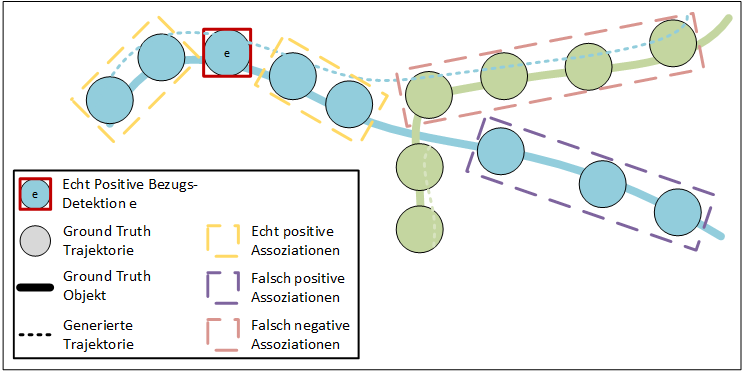
\includegraphics[width=\textwidth]{img/Grafiken/HOTA Assoziationsfehlerkonzept.png}
    \caption{Assoziationsfehlerkonzept der HOTA Metrik. \cite{HOTA}}
    \label{fig:KonzeptAssHOTA}
\end{figure}

Mit diesen Definitionen lässt sich die \gls{HOTA} Metrik berechnen. Für ein Element \(e \in \gls{EP}\) lässt sich ein \gls{Assoziation}[s]wert \(A(e)\) ermitteln. Über diesen und das \gls{Detektion}[sergebnis] lässt sich die \gls{HOTA} Wertung ermitteln. Dies zeigen die Gleichungen \ref{eq:HOTAalpha} und \ref{eq:AssScore}.

\begin{equation}
    \label{eq:HOTAalpha}
    HOTA_{\alpha} = \sqrt{\frac{\sum_{e \in EP} A(e)}{|EP| + |FN| + |FP|}}
\end{equation}

\begin{equation}
    \label{eq:AssScore}
    A(e) = \frac{|EPA(e)|}{|EPA(e)| + |FNA(e)| + |FPA(e)|}
\end{equation}

Da die Zuordnung mit einer Anforderung \(\alpha\) an die \gls{Lokalisation} stattfindet, wird diese Abhängigkeit der \(HOTA_{\alpha}\) Wertung in der \autoref{eq:HOTAalpha} über den Index verdeutlicht. Um die \gls{Lokalisation} mit in eine Gesamtwertung zu integrieren, wird die Ähnlichkeitsanforderung \(\alpha\) von 0 bis 1 variiert. Anschließend wird über diesen Verlauf der \(HOTA_{\alpha}\) Werte integriert, um eine \(\alpha\) unabhängige \gls{HOTA} Wertung zu erhalten. In der Praxis wird \(HOTA_{\alpha}\) für \(0.05 \leq \alpha \leq 0.95\) berechnet und über die Anzahl der Inkremente gemittelt. Dabei wird \(\alpha\) in Schritten von 0.05 inkrementiert. Die \autoref{eq:HOTA} zeigt die Berechnung der \gls{HOTA} Wertung.

\begin{equation}
    \label{eq:HOTA}
    HOTA = \int_{0}^{1} HOTA_{\alpha} d\alpha \approx \frac{1}{19} \sum_{\alpha \in (0,05, 0,1, \dots, 0,9, 0,95)} HOTA_{\alpha}
\end{equation}

Die Zuordnung des \gls{Tracking}[ergebnisses] zur \gls{Ground Truth} wird so optimiert, dass der \gls{HOTA} Wert maximal wird. Dies erfolgt so, dass die ungarische Methode als erstes Kriterium  \(|\gls{EP}|\) maximiert. Als zweites Kriterium wird der Mittelwert von \(A\) maximiert für \(\forall e \in \gls{EP}, A(e)\). Das dritte Kriterium maximiert die mittlere Ähnlichkeit \(s\) über alle \(\forall e \in \gls{EP}, s(e)\). \par
 
 \begin{wrapfigure}{l}{0.5\textwidth}
    \begin{center}
        \vspace*{-5mm}
        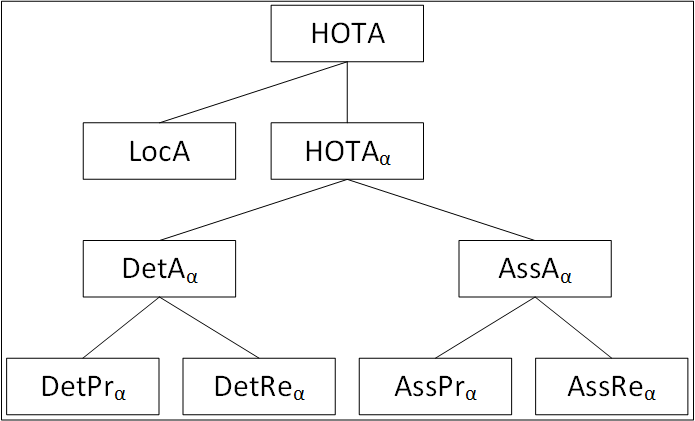
\includegraphics[width=0.5\textwidth]{img/Grafiken/HOTA Submetriken Pyramide.png}
        \vspace*{-10mm}
        \caption{Übersicht über den Zusammenhang der HOTA Submetriken. \cite{HOTA}}
        \label{fig:HOTASubmetrikPyram}
    \end{center}
\end{wrapfigure}

 Der \gls{HOTA} Wert lässt sich in Submetriken zerlegen. Dies ermöglicht eine ausführliche Einsicht in die unterschiedlichen \gls{Modul}[e] eines \gls{MOT} Systems. Die Abbildung \ref{fig:HOTASubmetrikPyram} zeigt den Zusammenhang von \gls{HOTA} und seinen Submetriken. \par 

Die Genauigkeit der \glsdisp{Lokalisationsfehler}{Lokalisation} lässt sich über die \gls{LocA} beurteilen. Dies wird nach Formel \ref{eq:LocA} berechnet.

\begin{equation}
    \label{eq:LocA}
    LocA = \int_{0}^{1} \frac{1}{|EP_{\alpha}|} \sum_{e \in (EP_{\alpha})} S(e) d\alpha
\end{equation}
\\
Die Genauigkeit der \gls{Detektion} ist beurteilbar über die \gls{DetA}. Die Rechenvorschrift zeigt die Formel \ref{eq:DetA}.

\begin{equation}
    \label{eq:DetA}
    DetA = \int_{0}^{1} \frac{|EP_{\alpha}|}{|FP_{\alpha}| + |FN_{\alpha}| + |EP_{\alpha}| d\alpha}
\end{equation}

Die Formel \ref{eq:AssA} zeigt die Berechnung der Genauigkeit der \gls{Assoziation}. Sie wird ausgedrückt über die \gls{AssA}. 

\begin{equation}
    \label{eq:AssA}
    AssA = \int_{0}^{1} \frac{1}{|EP_{\alpha}|} \sum_{e \in (EP_{\alpha})} A(e) d\alpha
\end{equation}

Wie man an den Formeln \ref{eq:DetA} und \ref{eq:AssA} sieht, setzt sich die Berechnung von \(\gls{HOTA}_{\alpha}\) (\autoref{eq:HOTAalpha}) aus dem geometrischen Mittelwert von \gls{DetA} und \gls{AssA} zusammen. Dies zeigt Formel \ref{eq:HOTAalphaGeoMean}.

\begin{equation}
\begin{split}
    \label{eq:HOTAalphaGeoMean}
    HOTA_{\alpha} &= \sqrt{\frac{\sum_{e \in EP} A(e)}{|EP| + |FN| + |FP|}} \\ 
    &= \sqrt{\frac{|EP_{\alpha}|}{|FP_{\alpha}| + |FN_{\alpha}| + |EP_{\alpha}|} \cdot \frac{1}{|EP_{\alpha}|} \sum_{e \in (EP_{\alpha})} A(e)} \\ 
    &= \sqrt{DetA_{\alpha} \cdot AssA_{\alpha}}
\end{split}
\end{equation}

Dies gewährleistet, dass die \gls{Detektion} und die \gls{Assoziation} gleichwertig in das Ergebnis einfließen. \par

Die \gls{DetA} Wertung lässt sich weiter zerlegen in Präzision \gls{DetPr} und Erkennungsrate \gls{DetRe}. Mit dem \gls{DetPr} Wert lässt sich beurteilen, wie viele falsch positive \gls{Detektion}[en] im \gls{Tracking}[ergebnis] vorhanden sind und mit dem \gls{DetRe} Wert ist die Anzahl der falsch negativen \gls{Detektion}[en] zu evaluieren. Die Formeln \ref{eq:DetPr} und \ref{eq:DetRe} zeigen die Berechnung von \gls{DetPr} und \gls{DetRe}. Die Formel \ref{eq:DetAfromPrRe} zeigt, wie sich \gls{DetA} daraus zusammensetzt \cite{HOTA}.

\begin{equation}
    \label{eq:DetPr}
    DetPr_{\alpha} = \frac{|EP|}{|EP| + |FP|}
\end{equation}

\begin{equation}
    \label{eq:DetRe}
    DetRe_{\alpha} = \frac{|EP|}{|EP| + |FN|}
\end{equation}

\begin{equation}
    \label{eq:DetAfromPrRe}
    DetA_{\alpha} = \frac{ DetRe_{\alpha} \cdot DetPr_{\alpha} }{ DetRe_{\alpha} + DetPr_{\alpha} -  DetRe_{\alpha} \cdot DetPr_{\alpha}}
\end{equation}

Ähnliches gilt für die \gls{AssA} Wertung. Diese lässt sich ebenfalls in einen  Präzisionswert \gls{AssPr} und eine Erkennungsrate \gls{AssRe} zerlegen. Der \gls{AssPr} Wert lässt Rückschlüsse auf die Menge an \gls{Merging Fehler} zu, die das \gls{MOT} System macht. Der \gls{AssRe} Wert ermögliche eine Beurteilung der Menge an \glsdisp{Fragmentation}{Fragmentationsfehlern} (\autoref{sec:MOT Fehlertypen}). Die Formeln \ref{eq:AssPr} und \ref{eq:AssRe} zeigen die Berechnung von \gls{AssPr} und \gls{AssRe}. Die Formel \ref{eq:AssAfromPrRe} zeigt, wie sich \gls{AssA} daraus zusammensetzt \cite{HOTA}. 

\begin{equation}
    \label{eq:AssPr}
    AssPr_{\alpha} =  \frac{1}{|EP_{\alpha}|} \sum_{e \in (EP)} \frac{|EPA(e)|}{|EPA(e)| + |FPA(e)|}
\end{equation}

\begin{equation}
    \label{eq:AssRe}
    AssRe_{\alpha} = \frac{1}{|EP_{\alpha}|} \sum_{e \in (EP)} \frac{|EPA(e)|}{|EPA(e)| + |FNA|(e)}
\end{equation}

\begin{equation}
    \label{eq:AssAfromPrRe}
    AssA_{\alpha} = \frac{AssRe_{\alpha} \cdot AssPr_{\alpha} }{AssRe_{\alpha} + AssPr_{\alpha} - AssRe_{\alpha} \cdot AssPr_{\alpha}}
\end{equation}

Die \textit{\gls{HOTA}} Metrik ist ein mächtiges Werkzeug, um \gls{MOT} Systeme zu vergleichen, da alle Aspekte in einem Gesamtwert berücksichtigt werden. Ebenfalls ermöglicht die Metrik ausführlichen Einblick in die Fehler von \gls{MOT} Systemen. Damit lassen sich stärken und schwächen von Systemen besser analysieren, als mit den \textit{\acrshort{CLEAR} \gls{MOT}} Metriken oder mit der \textit{\gls{IDF1}-Metrik} \cite{HOTA}. 